\section{Neutrino Beam Flux and Uncertainties}\label{sec:nu-osc-04}
%{\it Assigned to:} {\bf Laura Fields} with contributions from Zarko Pavlovic and Luke Pickering.
\label{sec:physics-lbnosc-flux}

The neutrino fluxes are described in detail in Section~\ref{sec:tools-mc-flux}.  They were generated using G4LBNF, a \textsc{Geant}4\xspace-based simulation of the LBNF neutrino beam.  The simulation is configured to use a detailed description of the \dword{lbnf} optimized beam design~\cite{optimizedbeamcdr}, which includes horns and target designed to maximize sensitivity to \dword{cpv} given the physical constraints on the beamline design.   

\begin{dunefigure}[Neutrino fluxes at the far detector]{fig:flux_flavor}
{Neutrino fluxes at the \dword{fd} for neutrino mode (left) and
antineutrino mode (right). }
    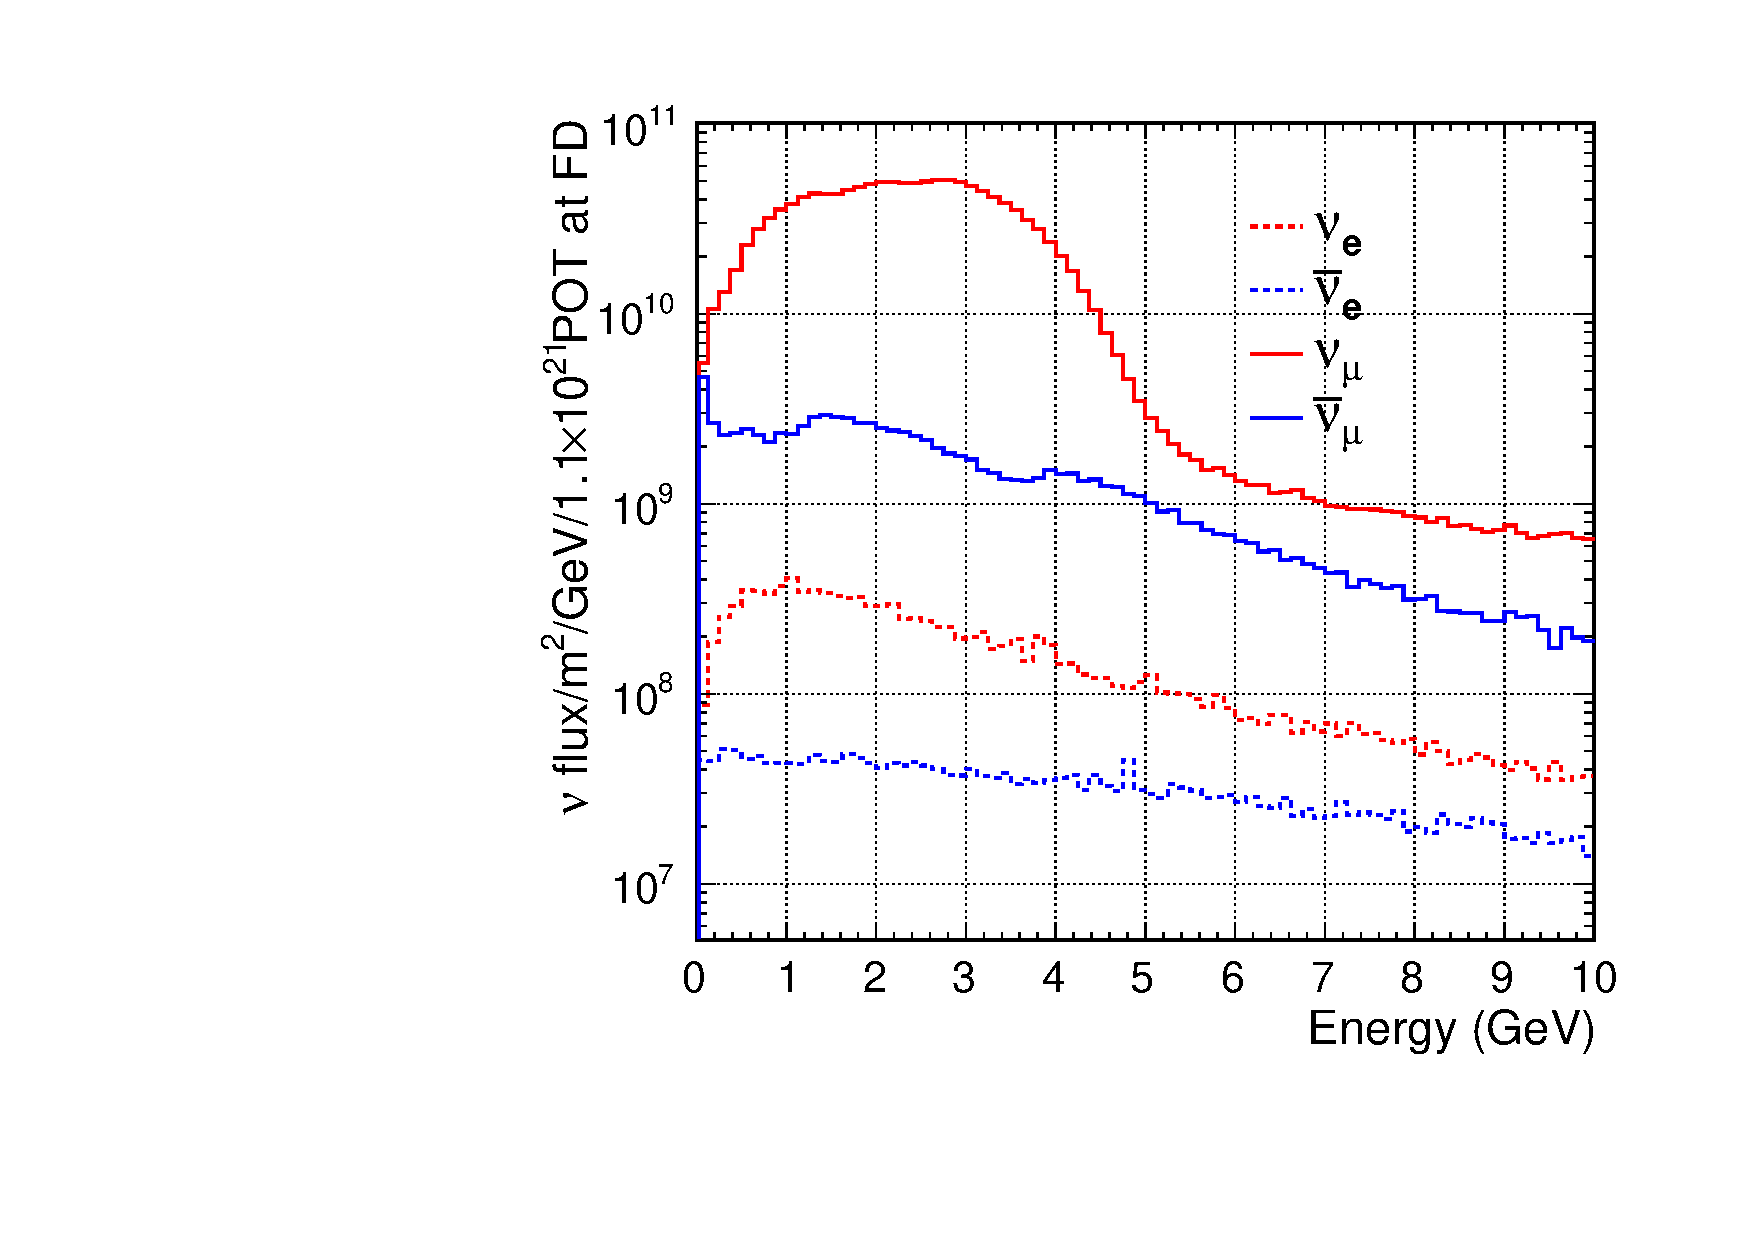
\includegraphics[width=0.45\textwidth]{dune_neutrino_fd_log.pdf}
     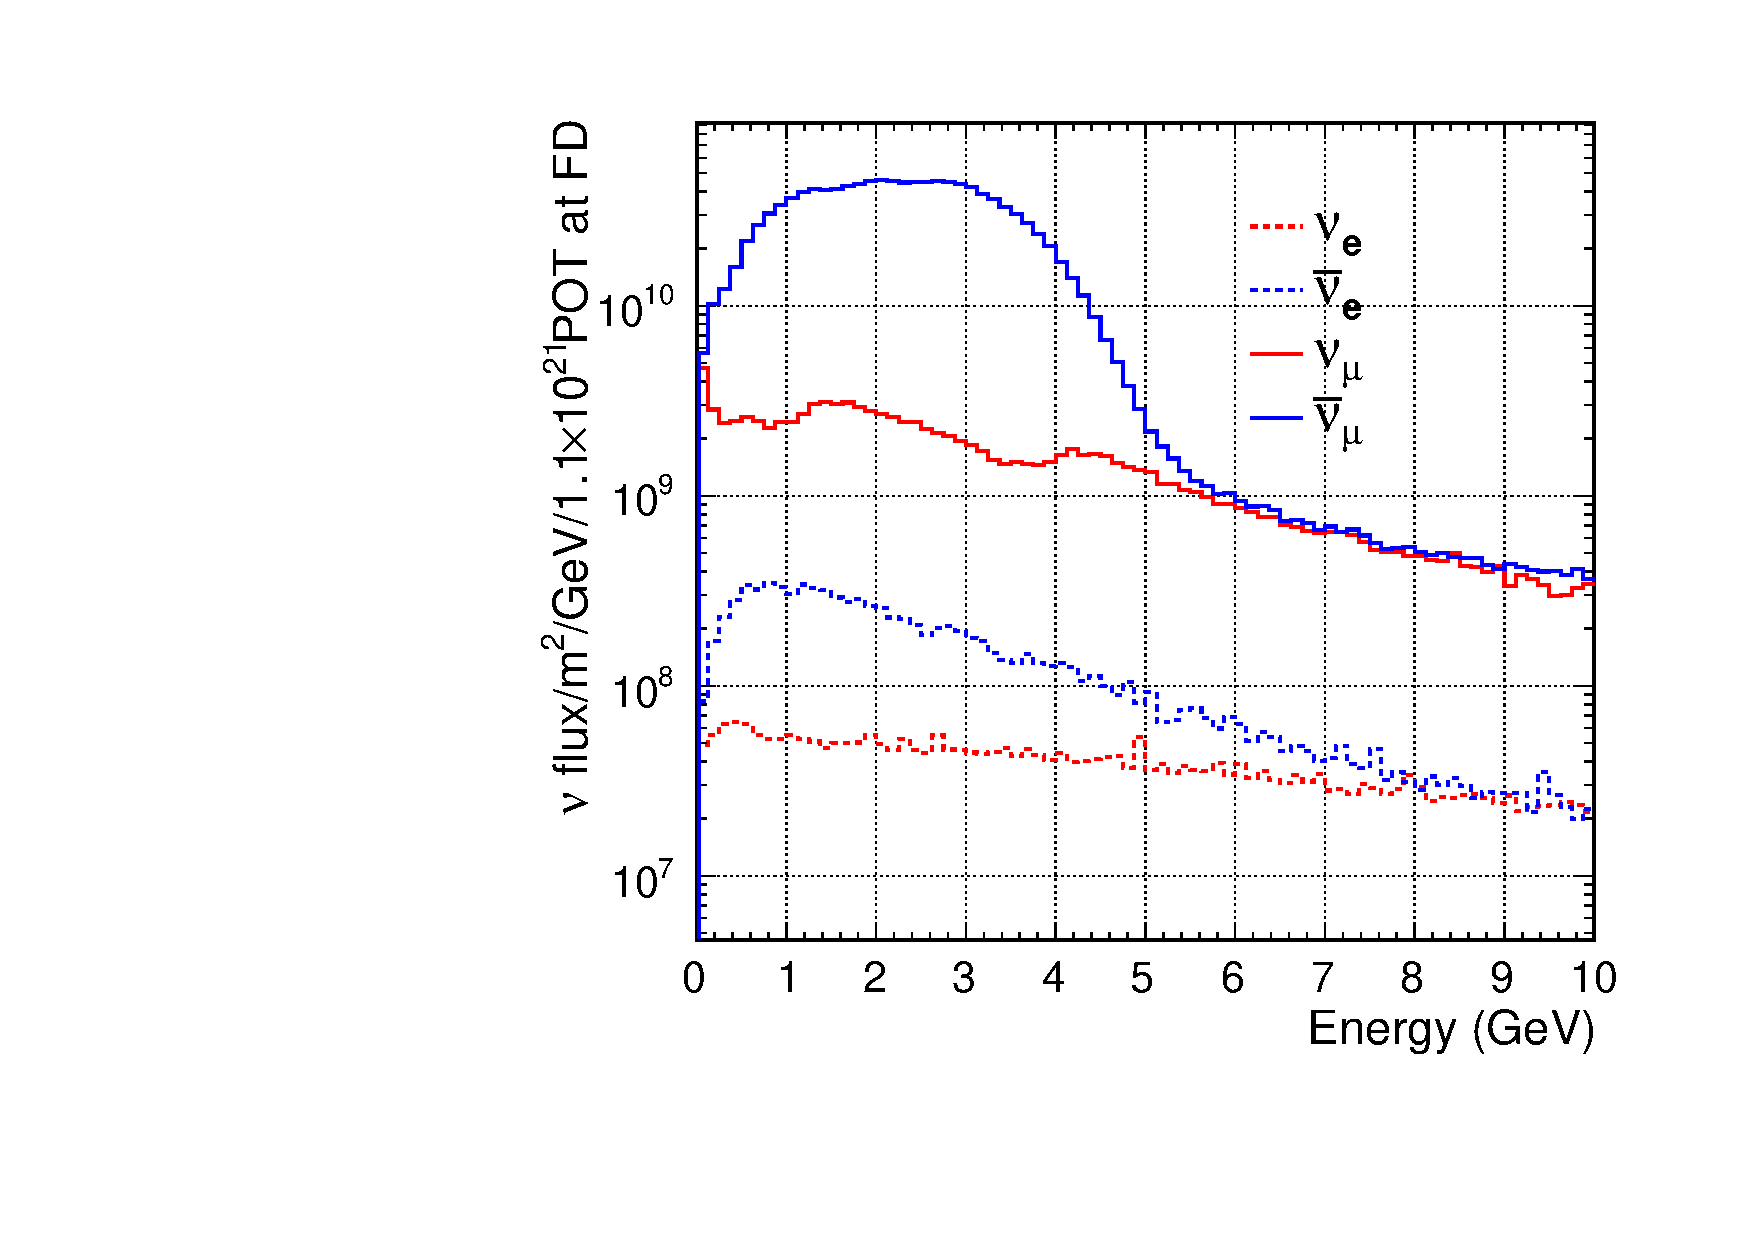
\includegraphics[width=0.45\textwidth]{dune_antineutrino_fd_log.pdf}
\end{dunefigure}

Neutrino fluxes for neutrino and antineutrino mode configurations of \dword{lbnf} are shown in Figure~\ref{fig:flux_flavor}.   Uncertainties on the neutrino fluxes arise primarily from uncertainties in hadrons produced off the target and uncertainties in the design parameters of the beamline, such as horn currents and horn and target positioning (commonly called ``focusing uncertainties''). Given current measurements of hadron production and LBNF estimates of alignment tolerances, flux uncertainties are approximately 8\% at the first oscillation maximum and 12\% at the second.  These uncertainties are highly correlated across energy bins and neutrino flavors

 Future hadron production measurements are expected to improve the quality of and the resulting constraints on these flux uncertainty estimates.  Approximately 40\% of the interactions that produce neutrinos in the LBNF beam simulation have no data constraints whatsoever.  Large uncertainties are assumed for these interactions. The largest unconstrained sources of uncertainty are proton quasielastic interactions and meson incident interactions.  The proposed EMPHATIC experiment at Fermilab will be able to constrain quasielastics and low energy interactions that dominate the lowest neutrino energy bins.  The NA61 experiment at CERN has taken data that will constrain many higher energy interactions, including meson incident, and also plans to measure hadrons produced off of a replica LBNF target, which would provide tight constraints on all interactions occurring in the target.  A similar program at NA61 has reduced flux uncertainties for T2K from ~10\% to ~5\%~\cite{Vladisavljevic:2018prd}, and NOvA is currently analyzing NA61 replica target data~\cite{Aduszkiewicz:2222876}.  Another proposed experiment, the LBNF spectrometer, would measure hadrons after both production and focusing in the horns, effectively constraining nearly all hadron production uncertainties, and could also enable measurement of the impact on focused hadrons of shifted alignment parameters (which is currently taken from simulations).  
The neutrino flux uncertainties, as well as their bin-to-bin and  flavor-to-flavor correlations, are very sensitive correlations in hadron production measurements.  None of the currently available measurements have provided correlations, so the uncertainty estimates make basic assumptions that statistical uncertainties are not correlated between bins but systematic uncertainties are completely correlated.  New hadron production measurements that cover phase space similar to past measurements but that provide bin-to-bin correlations would also improve the quality of the estimated neutrino flux uncertainties at DUNE.     

The unoscillated fluxes at the \dword{nd} and \dword{fd} are similar, but not identical (since the ND sees a line source, while the FD sees a point source. The relationship is well understood, and flux uncertainties mostly cancel for the ratio of fluxes between the two detectors.  Uncertainties on the ratio are around 1\% or smaller except at the falling edge of the focusing peak, where they rise to 2\%.    

The peak energy of neutrino flux falls off and the width of the peak narrows as the distance from the beams central axis increases. The flux at these ``off-axis'' positions can be understood though the relationship between the parent pion energy and neutrino energy, as shown in Figure~\ref{fig:OAAFluxFigs}. For an off-axis angle relative to the initial beam direction, the subsequent neutrino energy spectra is narrower and peaked at a lower energy than the on-axis spectra. At $575\,\textrm{m}$, the location of the \dword{nd} hall, a lateral shift of $1\,\textrm{m}$ corresponds to approximately a $0.1^\circ$ change in off-axis angle.

\begin{dunefigure}[Off-axis neutrino energy spectra and fluxes]{fig:OAAFluxFigs}
{(a) The neutrino energy as a function of parent pion energy for different angles away from the pion momentum vector. Figure from Ref.~\cite{Duffy:2016owt}. (b) The \dword{dune} \dword{nd} flux predictions over a range of off-axis positions for a \dword{nd} at $575\,\textrm{m}$ downstream of the upstream end of the first focusing horn. }
%is subfig package included? I don't think subfloat is working (ZP)
%  \subfloat[C][Off-axis pion decay kinematics]{
    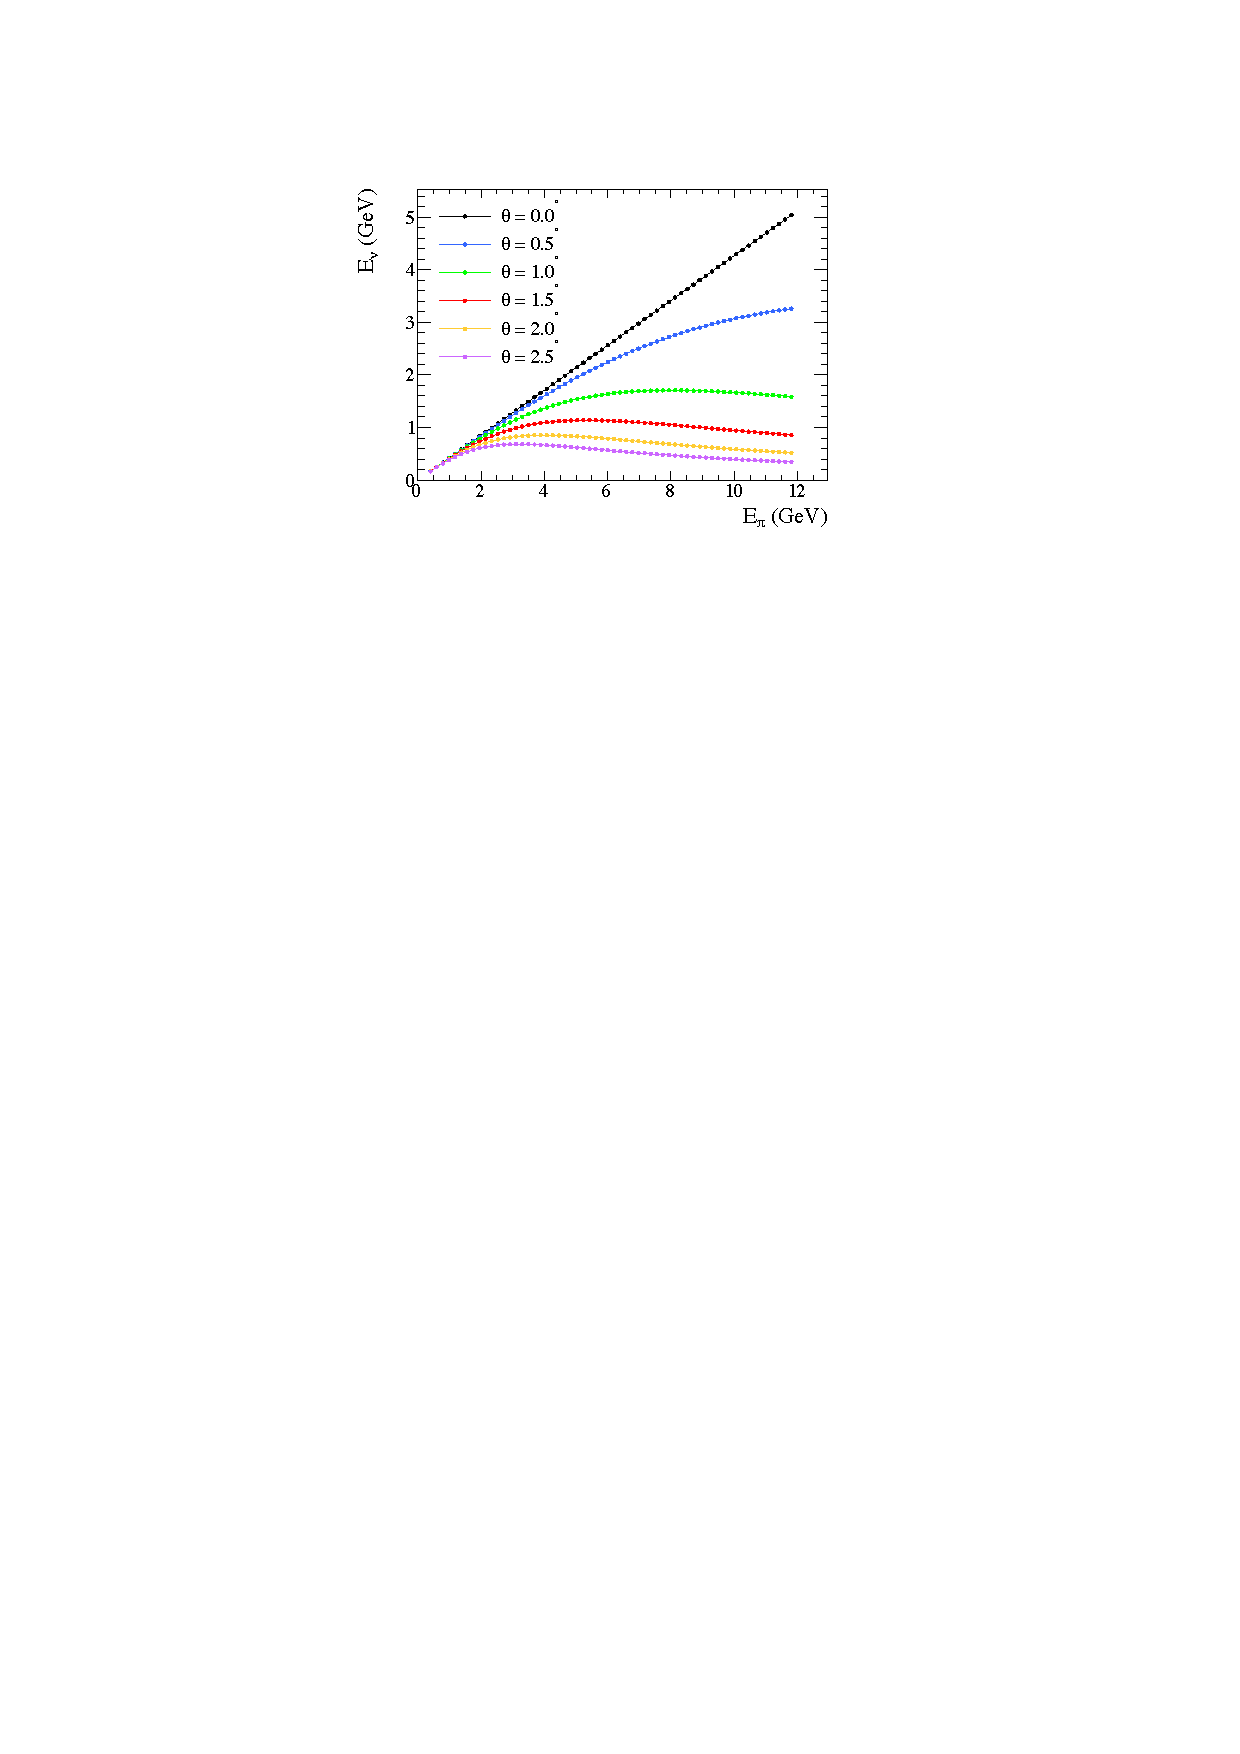
\includegraphics[width=0.4\textwidth]{OATrick.pdf}
%    \label{fig:OATrick}
%  }
%  \subfloat[][DUNE near detector flux predictions]{
    \raisebox{0.5em}{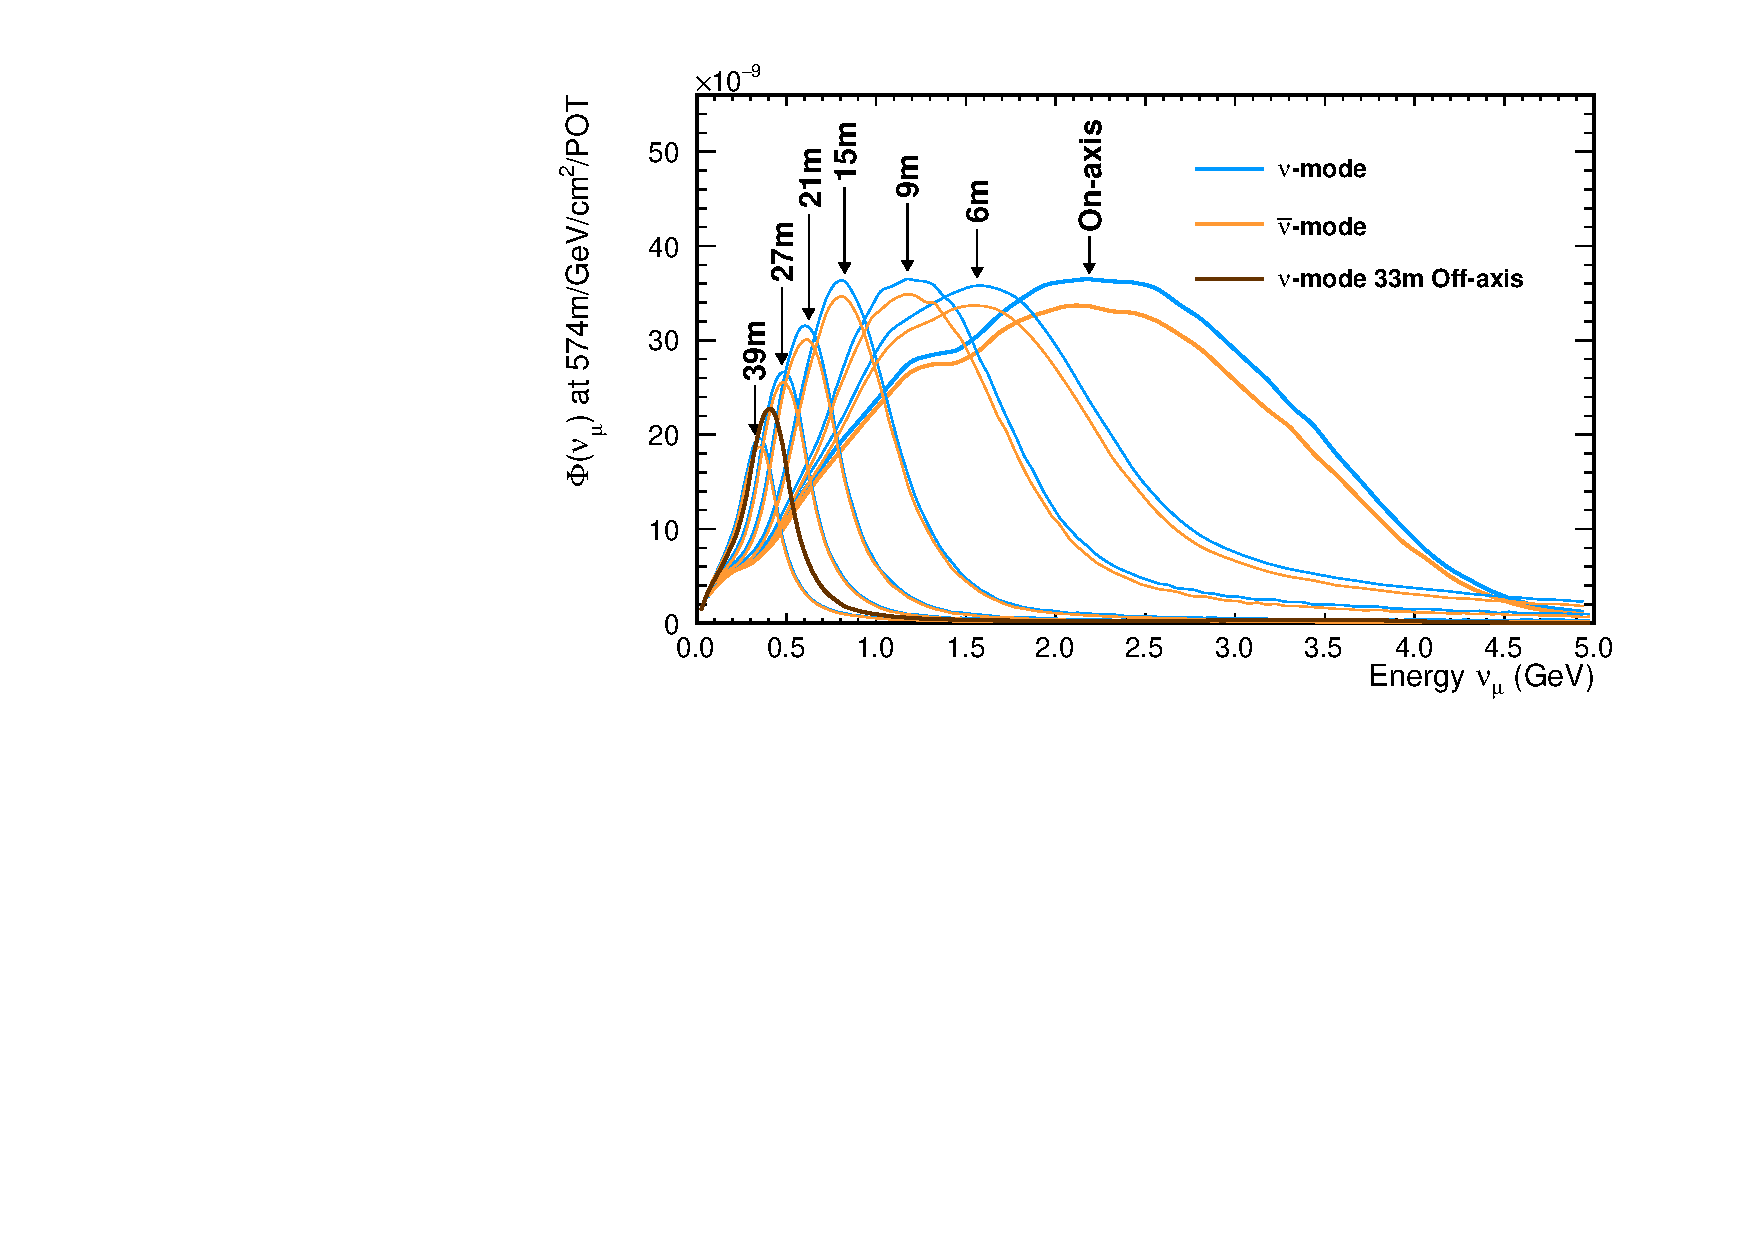
\includegraphics[width=0.45\textwidth]{dune_numu_offaxis_flux.pdf}}
%    \label{fig:OffAxisFluxes_1D}
%  }
\end{dunefigure}

The same sources of systematic uncertainty which affect the on-axis spectra also modify the off-axis spectra.  Generally, the size of the off-axis uncertainties is comparable to the on-axis uncertainties and the uncertainties are highly correlated across off-axis and on-axis positions. Studies of extreme changes to horn positions and current indicate that the larger than expected shifts to the horn focusing elements (as has been historically seen in \dword{numi}) would induce significant changes off-axis. Therefore, off-axis flux measurements are useful to diagnose beamline aberrations, and to further constrain flux uncertainties.

